\documentclass[times]{beamer}
\usepackage{amssymb}
\usepackage{amsmath}
\usepackage{amsfonts}
\usepackage{lmodern} 
% Calligraphic fonts
\newcommand{\calA}{{\cal A}}
\newcommand{\calB}{{\cal B}}
\newcommand{\calC}{{\cal C}}
\newcommand{\calD}{{\cal D}}
\newcommand{\calE}{{\cal E}}
\newcommand{\calF}{{\cal F}}
\newcommand{\calG}{{\cal G}}
\newcommand{\calH}{{\cal H}}
\newcommand{\calI}{{\cal I}}
\newcommand{\calJ}{{\cal J}}
\newcommand{\calK}{{\cal K}}
\newcommand{\calL}{{\cal L}}
\newcommand{\calM}{{\cal M}}
\newcommand{\calN}{{\cal N}}
\newcommand{\calO}{{\cal O}}
\newcommand{\calP}{{\cal P}}
\newcommand{\calQ}{{\cal Q}}
\newcommand{\calR}{{\cal R}}
\newcommand{\calS}{{\cal S}}
\newcommand{\calT}{{\cal T}}
\newcommand{\calU}{{\cal U}}
\newcommand{\calV}{{\cal V}}
\newcommand{\calW}{{\cal W}}
\newcommand{\calX}{{\cal X}}
\newcommand{\calY}{{\cal Y}}
\newcommand{\calZ}{{\cal Z}}

% Sets:
\newcommand{\setA}{\textsf{A}}
\newcommand{\setB}{\textsf{B}}
\newcommand{\setC}{\textsf{C}}
\newcommand{\setD}{\textsf{D}}
\newcommand{\setE}{\textsf{E}}
\newcommand{\setF}{\textsf{F}}
\newcommand{\setG}{\textsf{G}}
\newcommand{\setH}{\textsf{H}}
\newcommand{\setI}{\textsf{I}}
\newcommand{\setJ}{\textsf{J}}
\newcommand{\setK}{\textsf{K}}
\newcommand{\setL}{\textsf{L}}
\newcommand{\setM}{\textsf{M}}
\newcommand{\setN}{\textsf{N}}
\newcommand{\setO}{\textsf{O}}
\newcommand{\setP}{\textsf{P}}
\newcommand{\setQ}{\textsf{Q}}
\newcommand{\setR}{\textsf{R}}
\newcommand{\setS}{\textsf{S}}
\newcommand{\setT}{\textsf{T}}
\newcommand{\setU}{\textsf{U}}
\newcommand{\setV}{\textsf{V}}
\newcommand{\setW}{\textsf{W}}
\newcommand{\setX}{\textsf{X}}
\newcommand{\setY}{\textsf{Y}}
\newcommand{\setZ}{\textsf{Z}}

% Vectors
\newcommand{\bfa}{\mathbf{a}}
\newcommand{\bfb}{\mathbf{b}}
\newcommand{\bfc}{\mathbf{c}}
\newcommand{\bfd}{\mathbf{d}}
\newcommand{\bfe}{\mathbf{e}}
\newcommand{\bff}{\mathbf{f}}
\newcommand{\bfg}{\mathbf{g}}
\newcommand{\bfh}{\mathbf{h}}
\newcommand{\bfi}{\mathbf{i}}
\newcommand{\bfj}{\mathbf{j}}
\newcommand{\bfk}{\mathbf{k}}
\newcommand{\bfl}{\mathbf{l}}
\newcommand{\bfm}{\mathbf{m}}
\newcommand{\bfn}{\mathbf{n}}
\newcommand{\bfo}{\mathbf{o}}
\newcommand{\bfp}{\mathbf{p}}
\newcommand{\bfq}{\mathbf{q}}
\newcommand{\bfr}{\mathbf{r}}
\newcommand{\bfs}{\mathbf{s}}
\newcommand{\bft}{\mathbf{t}}
\newcommand{\bfu}{\mathbf{u}}
\newcommand{\bfv}{\mathbf{v}}
\newcommand{\bfw}{\mathbf{w}}
\newcommand{\bfx}{\mathbf{x}}
\newcommand{\bfy}{\mathbf{y}}
\newcommand{\bfz}{\mathbf{z}}


\newcommand{\bfalpha}{\boldsymbol{\alpha}}
\newcommand{\bfbeta}{\boldsymbol{\beta}}
\newcommand{\bfgamma}{\boldsymbol{\gamma}}
\newcommand{\bfdelta}{\boldsymbol{\delta}}
\newcommand{\bfepsilon}{\boldsymbol{\epsilon}}
\newcommand{\bfzeta}{\boldsymbol{\zeta}}
\newcommand{\bfeta}{\boldsymbol{\eta}}
\newcommand{\bftheta}{\boldsymbol{\theta}}
\newcommand{\bfiota}{\boldsymbol{\iota}}
\newcommand{\bfkappa}{\boldsymbol{\kappa}}
\newcommand{\bflambda}{\boldsymbol{\lambda}}
\newcommand{\bfmu}{\boldsymbol{\mu}}
\newcommand{\bfnu}{\boldsymbol{\nu}}
\newcommand{\bfomicron}{\boldsymbol{\omicron}}
\newcommand{\bfpi}{\boldsymbol{\pi}}
\newcommand{\bfrho}{\boldsymbol{\rho}}
\newcommand{\bfsigma}{\boldsymbol{\sigma}}
\newcommand{\bftau}{\boldsymbol{\tau}}
\newcommand{\bfupsilon}{\boldsymbol{\upsilon}}
\newcommand{\bfphi}{\boldsymbol{\phi}}
\newcommand{\bfchi}{\boldsymbol{\chi}}
\newcommand{\bfpsi}{\boldsymbol{\psi}}
\newcommand{\bfomega}{\boldsymbol{\omega}}
\newcommand{\bfxi}{\boldsymbol{\xi}}
\newcommand{\bfell}{\boldsymbol{\ell}}

% Matrices
\newcommand{\bfA}{\mathbf{A}}
\newcommand{\bfB}{\mathbf{B}}
\newcommand{\bfC}{\mathbf{C}}
\newcommand{\bfD}{\mathbf{D}}
\newcommand{\bfE}{\mathbf{E}}
\newcommand{\bfF}{\mathbf{F}}
\newcommand{\bfG}{\mathbf{G}}
\newcommand{\bfH}{\mathbf{H}}
\newcommand{\bfI}{\mathbf{I}}
\newcommand{\bfJ}{\mathbf{J}}
\newcommand{\bfK}{\mathbf{K}}
\newcommand{\bfL}{\mathbf{L}}
\newcommand{\bfM}{\mathbf{M}}
\newcommand{\bfN}{\mathbf{N}}
\newcommand{\bfO}{\mathbf{O}}
\newcommand{\bfP}{\mathbf{P}}
\newcommand{\bfQ}{\mathbf{Q}}
\newcommand{\bfR}{\mathbf{R}}
\newcommand{\bfS}{\mathbf{S}}
\newcommand{\bfT}{\mathbf{T}}
\newcommand{\bfU}{\mathbf{U}}
\newcommand{\bfV}{\mathbf{V}}
\newcommand{\bfW}{\mathbf{W}}
\newcommand{\bfX}{\mathbf{X}}
\newcommand{\bfY}{\mathbf{Y}}
\newcommand{\bfZ}{\mathbf{Z}}


\newcommand{\bfGamma}{\boldsymbol{\Gamma}}
\newcommand{\bfDelta}{\boldsymbol{\Delta}}
\newcommand{\bfTheta}{\boldsymbol{\Theta}}
\newcommand{\bfLambda}{\boldsymbol{\Lambda}}
\newcommand{\bfPi}{\boldsymbol{\Pi}}
\newcommand{\bfSigma}{\boldsymbol{\Sigma}}
\newcommand{\bfUpsilon}{\boldsymbol{\Upsilon}}
\newcommand{\bfPhi}{\boldsymbol{\Phi}}
\newcommand{\bfPsi}{\boldsymbol{\Psi}}
\newcommand{\bfOmega}{\boldsymbol{\Omega}}


% Blackboard Bold:
\newcommand{\bbA}{\mathbb{A}}
\newcommand{\bbB}{\mathbb{B}}
\newcommand{\bbC}{\mathbb{C}}
\newcommand{\bbD}{\mathbb{D}}
\newcommand{\bbE}{\mathbb{E}}
\newcommand{\bbF}{\mathbb{F}}
\newcommand{\bbG}{\mathbb{G}}
\newcommand{\bbH}{\mathbb{H}}
\newcommand{\bbI}{\mathbb{I}}
\newcommand{\bbJ}{\mathbb{J}}
\newcommand{\bbK}{\mathbb{K}}
\newcommand{\bbL}{\mathbb{L}}
\newcommand{\bbM}{\mathbb{M}}
\newcommand{\bbN}{\mathbb{N}}
\newcommand{\bbO}{\mathbb{O}}
\newcommand{\bbP}{\mathbb{P}}
\newcommand{\bbQ}{\mathbb{Q}}
\newcommand{\bbR}{\mathbb{R}}
\newcommand{\bbS}{\mathbb{S}}
\newcommand{\bbT}{\mathbb{T}}
\newcommand{\bbU}{\mathbb{U}}
\newcommand{\bbV}{\mathbb{V}}
\newcommand{\bbW}{\mathbb{W}}
\newcommand{\bbX}{\mathbb{X}}
\newcommand{\bbY}{\mathbb{Y}}
\newcommand{\bbZ}{\mathbb{Z}}




\setbeamertemplate{navigation symbols}{}

\title{ECE 417/598: Pseudo-Inverse review}
\author{Vikas Dhiman}
\date{Feb 9, 2022}
\begin{document}
\begin{frame}
  \titlepage
  \end{frame}
  \begin{frame}
    
\includegraphics[width=\linewidth]{media/purity.png}
  \end{frame}

  \begin{frame}
    \begin{minipage}[b]{0.1\linewidth}\tiny{Robotics is applied everything}\\
      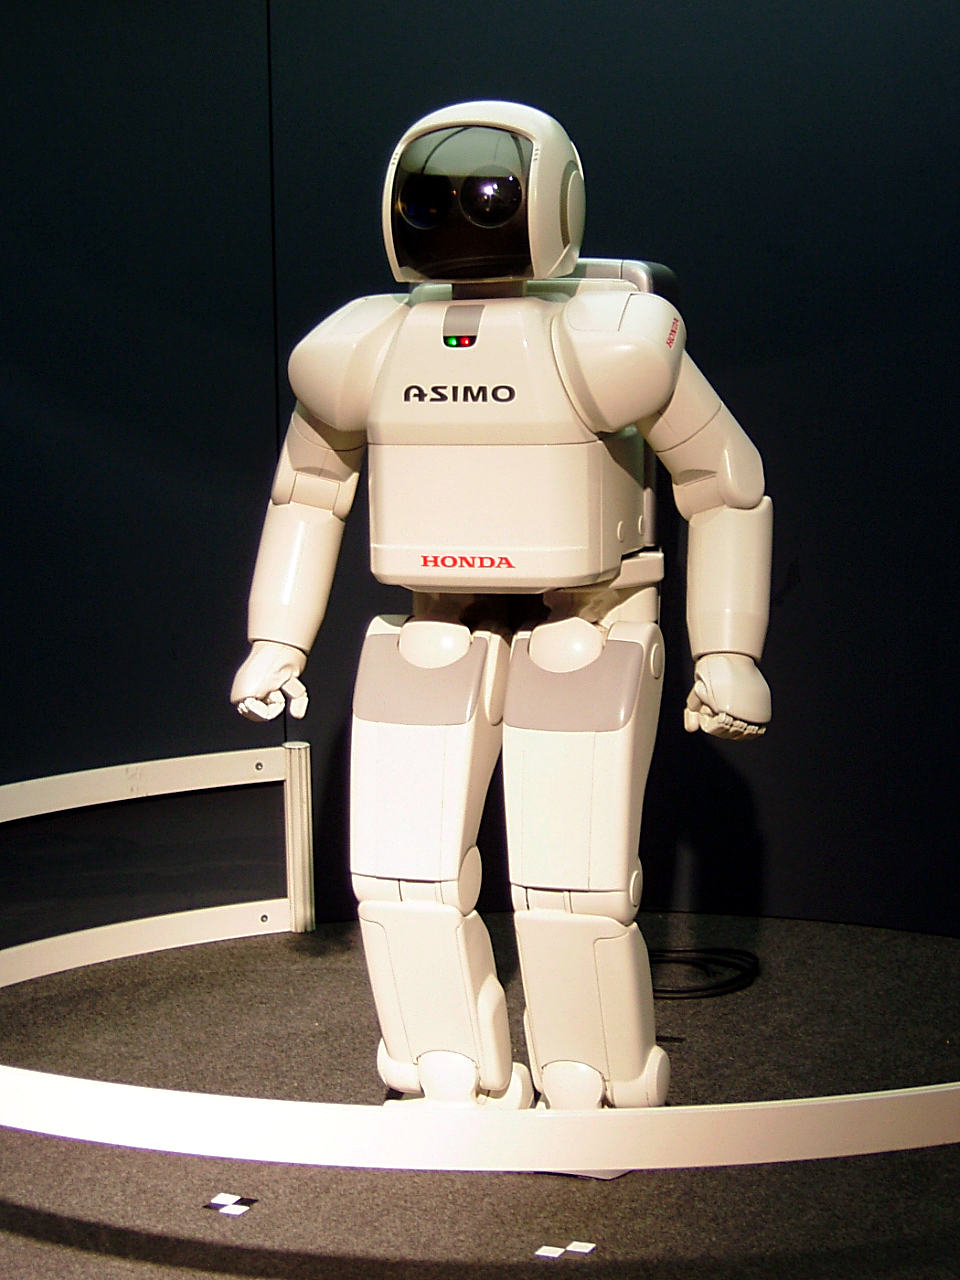
\includegraphics[width=\linewidth]{media/HONDA_ASIMO.jpg}\end{minipage}%
    \hspace{0.3\linewidth}
\includegraphics[width=0.5\linewidth]{media/purity.png}
  \end{frame}
  \begin{frame}
    \href{https://github.com/wecacuee/ECE417-Mobile-Robots}{Link to github}
    \end{frame}
  \begin{frame}{Pseudo-Inverse}
    \begin{align}
      \bfA \bfA^\dagger \bfA &=  \bfA \\
      \text{If SVD of $\bfA$ is given by } \bfA &= \bfU \Sigma \bfV^\top 
      \text{ then } \bfA^\dagger = \bfU \Sigma^{-1} \bfV^\top \\
      \text{if } \bfA \text{ is tall, then } \bfA^\dagger &= (\bfA^\top \bfA)^{-1} \bfA^\top \\
      \text{if } \bfA \text{ is fat, then } \bfA^\dagger &=  \bfA^\top (\bfA \bfA^\top)^{-1}
    \end{align}\footnote{See Appendix A of Gilbert Strang (1988): Linear Algebra
    and Its Applications}

  \end{frame}
  \begin{frame}{Pseudo-Inverse for tall matrix by Optimization}
    \begin{align}
      \min_{\bfx} &\|A\bfx - \bfb\|_2^2
                    \\
      &= \min_\bfx (A\bfx - \bfb)^\top (A\bfx - \bfb)
      \\
      &= \min_\bfx (\bfx^\top A^\top - \bfb^\top) (A\bfx - \bfb)
      \\
      &= \min_\bfx (\bfx^\top A^\top - \bfb^\top) (A\bfx - \bfb)
      \\
      &= \min_\bfx \bfx^\top A^\top A\bfx - \bfb^\top A\bfx - \bfx^\top A^\top \bfb + \bfb^\top \bfb
    \end{align}\footnote{Also see Chapter 3 of Gilbert Strang (1988): Linear Algebra
      and Its Applications}
  \end{frame}

  \begin{frame}

    Recall that a minimum (or maximum) point of a differentiable function $f(\bfx)$,
    $f'(\bfx)  = 0$. Let us define vector derivative as

    \begin{align}
      \frac{\partial f(\bfx)}{\partial \bfx} = \begin{bmatrix}
          \frac{\partial f(\bfx)}{\partial x_1}
            \\
            \frac{\partial f(\bfx)}{\partial x_2}
            \\
            \vdots
            \\
            \frac{\partial f(\bfx)}{\partial x_n}
          \end{bmatrix}
    \end{align}
    You can verfiy that
    \begin{align}
      \frac{\partial }{\partial \bfx} \bfx^\top Q \bfx &= 2 Q\bfx
      \\
      \frac{\partial }{\partial \bfx} \bfb^\top \bfx &= \bfb
      \end{align}
  \end{frame}

  \begin{frame}
    At a minimum point $\bfx$,
    \begin{align}
     &\frac{\partial }{\partial \bfx} \bfx^\top A^\top A\bfx - \bfb^\top A\bfx - \bfx^\top A^\top \bfb + \bfb^\top \bfb = 0
       \\
      \text{or } & 2A^\top A\bfx - 2 A^\top \bfb = 0
      \\
      \text{or } & \bfx = \underbrace{(A^\top A)^{-1} A^\top}_{A^\dagger} \bfb
    \end{align}
  \end{frame}

  \begin{frame}{Application }
    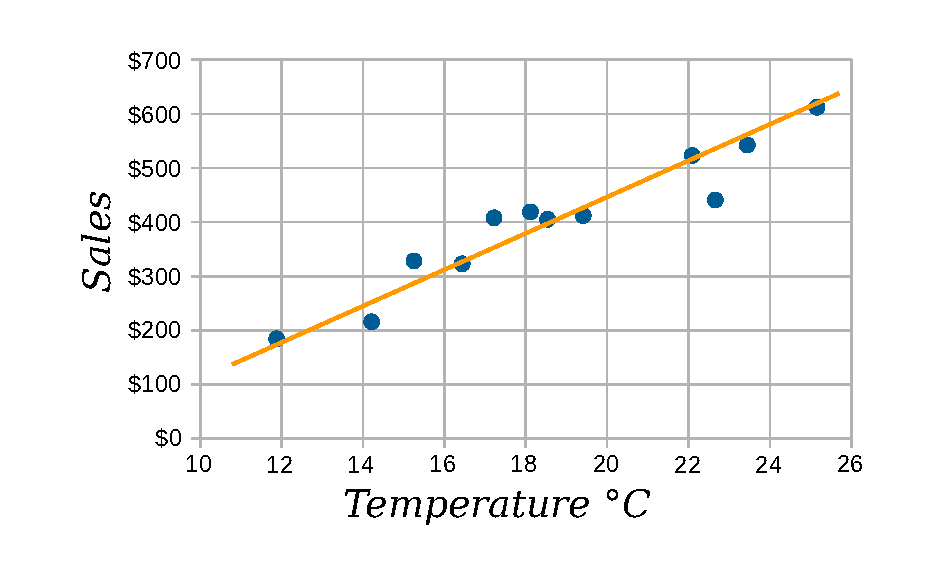
\includegraphics[width=\linewidth]{media/scatter-plot.pdf}
  \end{frame}
  \begin{frame}
    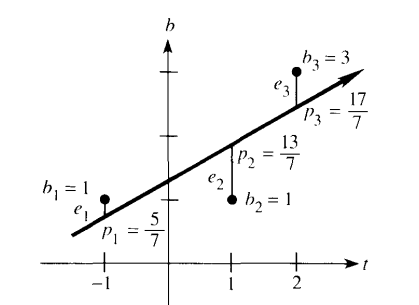
\includegraphics[width=0.5\linewidth]{media/straight-line-approx-gilbert-strang.png}
 \end{frame}


  \begin{frame}{Homogeneous representation of lines}
    \[ ax + by + c = 0\]
  \end{frame}

  \begin{frame}{Projective space}
    \[ \bbP^2 = \bbR^3 - (0, 0, 0)^\top \]
    \end{frame}

    \begin{frame}{Homogeneous representation of points}
      \[ ax + by + c = 0\]
    \end{frame}

    \begin{frame}{Eq of line in Projective space}
      The point $\bfx \in \bbP^2$ lies on a line $\bfl$ if and only if
      $\bfx^\top \bfl = 0$.
      \end{frame}
      \begin{frame}{Intersection of lines}
        \end{frame}

  \begin{frame}{Vanishing Point}
    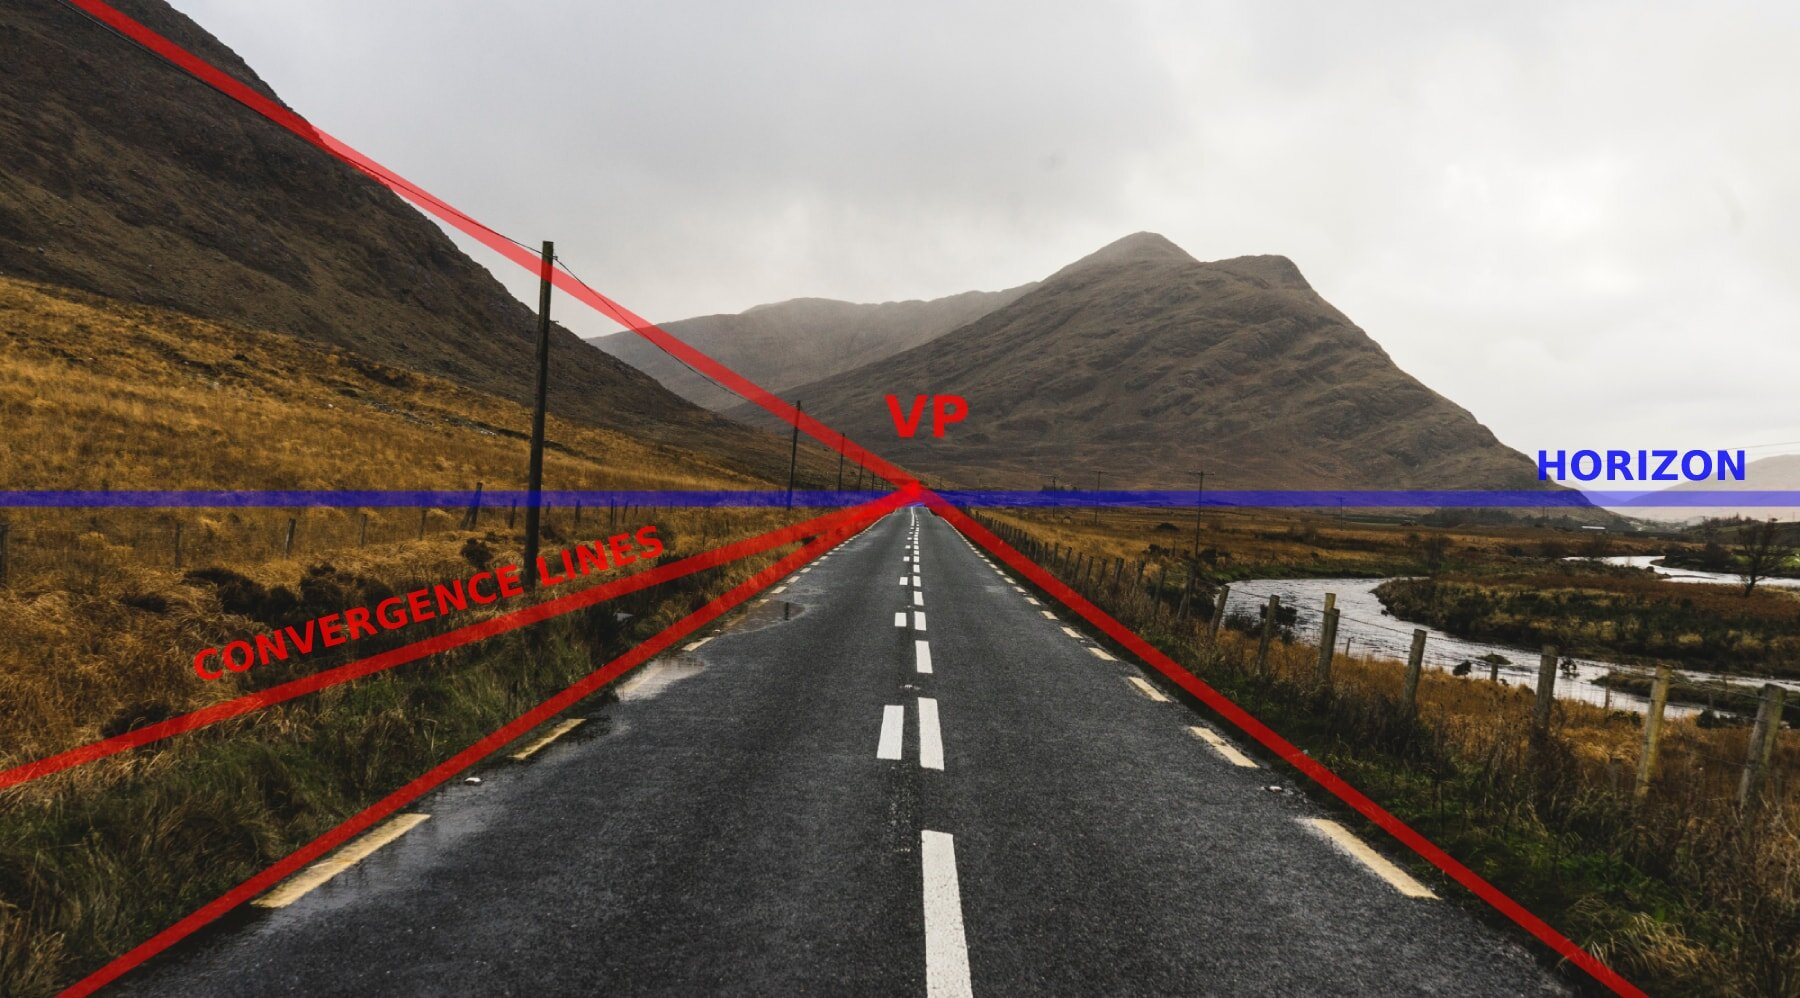
\includegraphics[width=0.7\linewidth]{media/vanishing-lines.jpeg}
    \\
    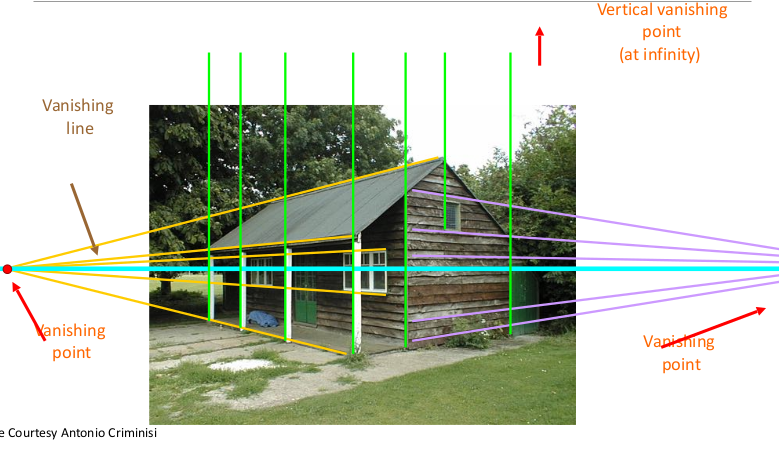
\includegraphics[width=0.7\linewidth]{media/vanishing-points.png}
  \end{frame}

  \begin{frame}{Vanishing Point}
    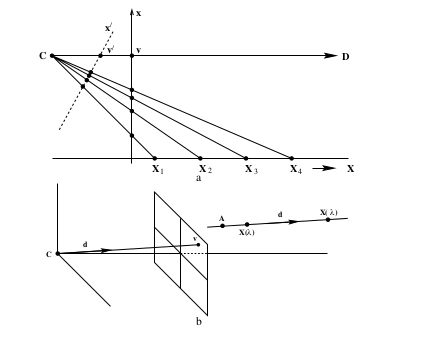
\includegraphics[width=0.5\linewidth]{media/vanishing-point-formation.png}
  \end{frame}

\end{document}